\subsection*{Graphics credits}
	% TODO: nice tabular showing images

\newcommand{\ccbythree}{\href{https://creativecommons.org/licenses/by/3.0/}{
\includegraphics[width=.15\textwidth]{cc-by.png}}}
\newcommand{\ccbysathree}{\href{https://creativecommons.org/licenses/by-sa/3.0/}{
\includegraphics[width=.15\textwidth]{CC-BY-SA_500.png}}}
\newcommand{\cczero}{\href{https://creativecommons.org/publicdomain/zero/1.0/}{
\includegraphics[width=.15\textwidth]{cc-zero.png}}}
\newcommand{\publicdomain}{
\includegraphics[width=.15\textwidth]{publicdomain.png}}

\begin{tabular}{| l | l | p{3.5cm} | p{3cm} | l |}
	\hline
	\textbf{Version} & \textbf{Image} & \textbf{Source} & \textbf{Author} & \textbf{License}
	%------------------------------------------------------------
	\\\hline
	\imitator{} & 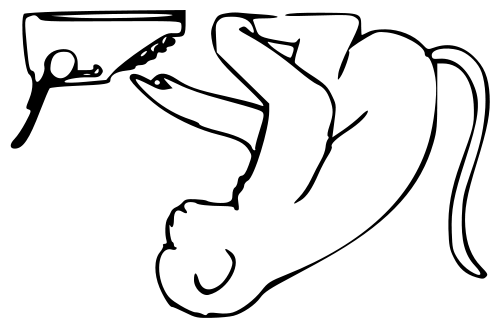
\includegraphics[width=.15\textwidth]{imitator-500.png} & \href{https://commons.wikimedia.org/wiki/File:Typing_monkey.svg}{\nolinkurl{Typing monkey.svg}} & KaterBegemot & \ccbysathree{}
	%------------------------------------------------------------
	\\\hline
	2.x versions & 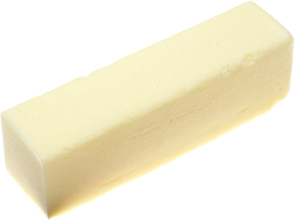
\includegraphics[width=.15\textwidth]{logo2-300.png} & \href{https://commons.wikimedia.org/wiki/File:Stick_of_butter.jpg}{\nolinkurl{Stick_of_butter.jpg}} & Renee Comet & \publicdomain{}
	%------------------------------------------------------------
	\\\hline
	version 2.7 & 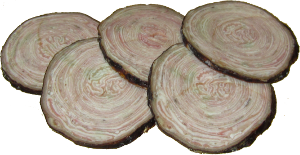
\includegraphics[width=.15\textwidth]{logo2-7-300.png} & \href{https://commons.wikimedia.org/wiki/File:Andouille-Scheiben.jpg}{\nolinkurl{Andouille-Scheiben.jpg}} & Pwagenblast & \ccbythree{}
	% NOTE: background erasing done by Fabrice Kordon
	%------------------------------------------------------------
	\\\hline
	version 2.8 & 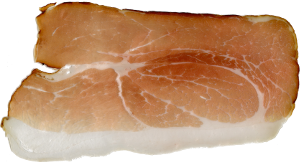
\includegraphics[width=.15\textwidth]{logo2-8-300.png} & \href{https://commons.wikimedia.org/wiki/File:Schinken-roh.jpg}{\nolinkurl{Schinken-roh.jpg}} & Rainer Zenz & \ccbythree{}
	%------------------------------------------------------------
	\\\hline
	version 2.9 & 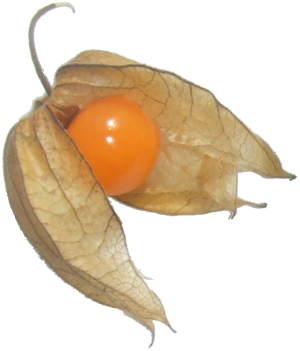
\includegraphics[width=.15\textwidth]{logo2-9-300.png} & \href{https://commons.wikimedia.org/wiki/File:Physalis_peruviana.jpg}{\nolinkurl{Physalis peruviana.jpg}} & Hans B.~commonswiki (assumed?) & \publicdomain{}
	%------------------------------------------------------------
	\\\hline
	version 2.10 & 
\includegraphics[width=.15\textwidth]{logo2-10-300.png} & \href{https://pixabay.com/fr/m%C3%A9duse-tentacules-medusa-marine-154799/}{méduses tentacules} & (?) & \cczero{}
	%------------------------------------------------------------
	\\\hline
	version 2.11 & 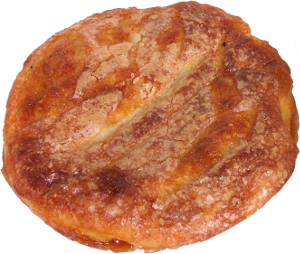
\includegraphics[width=.15\textwidth]{logo2-11-300.png} & \href{https://commons.wikimedia.org/wiki/File:Kouignamann.JPG}{Véritable Kouign Amann de Douarnenez} & Haltopub & \publicdomain{}
	%------------------------------------------------------------
	\\\hline
	version 2.12 & 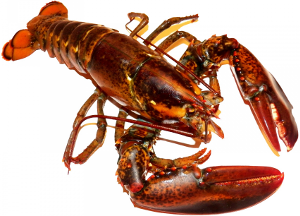
\includegraphics[width=.15\textwidth]{logo2-12-300.png} & \href{https://publicdomainpictures.net/en/view-image.php?image=39798&picture=lobster}{Photo of a live lobster} & Junior Libby & \cczero{}
	%------------------------------------------------------------
	\\\hline
\end{tabular}

% NOTE: logos can be downloaded at https://creativecommons.org/about/downloads/


% \paragraph{\imitator{}'s logo} comes from \stylePath{Typing monkey.svg} by KaterBegemot on Wikimedia Commons
% 	(License: Creative Commons Attribution-Share Alike 3.0 Unported).
% 
% \url{https://commons.wikimedia.org/wiki/File:Typing_monkey.svg}
% 
% 
% \paragraph{\imitator{}'s 2.x version logo} comes from \stylePath{Stick\_of\_butter.jpg} by Renee Comet on Wikimedia Commons
% 	(License: public domain).
% 
% \url{https://commons.wikimedia.org/wiki/File:Stick_of_butter.jpg}
% 
% \paragraph{\imitator{}'s 2.7 version logo} comes from \stylePath{Andouille-Scheiben.jpg} by Pwagenblast on Wikimedia Commons
% 	(License: Creative Commons Attribution 3.0 Unported).
% The background erasing was done by Fabrice~Kordon.
% 
% \url{https://commons.wikimedia.org/wiki/File:Andouille-Scheiben.jpg}
% 
% 
% \paragraph{\imitator{}'s 2.8 version logo} comes from \stylePath{Schinken-roh.jpg} by Rainer Zenz on Wikimedia Commons
% 	(License: Creative Commons Attribution-Share Alike 3.0 Unported).
% 
% \url{https://commons.wikimedia.org/wiki/File:Schinken-roh.jpg}
% 
% 
% \paragraph{\imitator{}'s 2.9 version logo} comes from \stylePath{Physalis peruviana.jpg} by Hans B.~commonswiki (assumed?) on Wikimedia Commons
% 	(License: public domain).
% 
% \url{https://commons.wikimedia.org/wiki/File:Physalis_peruviana.jpg}
%  
% 
% \paragraph{\imitator{}'s 2.10 version logo} comes from ``méduses tentacules'' by (?) on \url{pixabay.com}
% 	(License: CC0).
% 
% \url{https://pixabay.com/fr/m%C3%A9duse-tentacules-medusa-marine-154799/}
% 
% \paragraph{\imitator{}'s 2.11 version logo} comes from ``Véritable Kouign Amann de Douarnenez'' by Haltopub on Wikimedia Commons
% 	(License: public domain).
% 
% \url{https://commons.wikimedia.org/wiki/File:Kouignamann.JPG}
%  
% \paragraph{\imitator{}'s 2.12 version logo} comes from ``Photo of a live lobster'' by Junior Libby on PublicDomainPictures.net
% 	(License: CC0 - public domain).
% 
% \url{https://publicdomainpictures.net/en/view-image.php?image=39798&picture=lobster}
